\subsection{Product Perspective}
The system is going to be divided in three main components:
\begin{enumerate}
\item Mobile application version for phones and tablets.
\item Web browser version.
\item Backend structure to support the functioning of the service.
\end{enumerate}
While the backend structure is needed for the functioning of the service provided, only one of the two applications is required to interact with the system.\\
APIs for each component must be provided in order to allow future development and introduction of new functionalities like an automated system for buying tickets of public transportation vehicles.
\subsubsection*{Class Diagram}
In \autoref{fig:ClassDiagram0} is represented the class diagram of the basic components of the system to be, a more detailed one will be discussed later on.
\begin{figure}[h]
\centering
	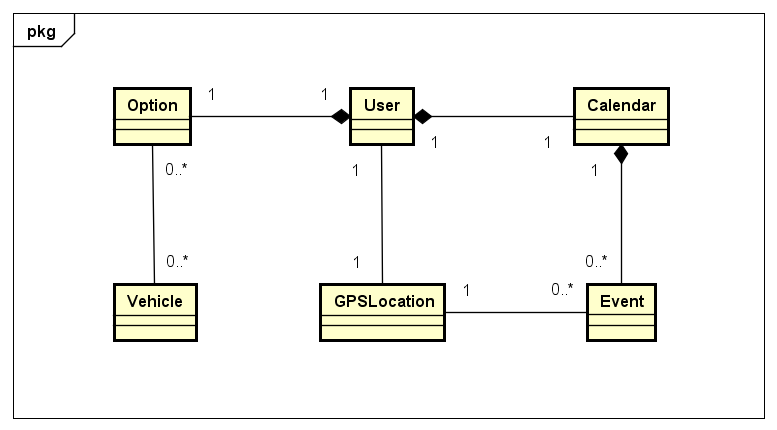
\includegraphics[width=\textwidth, keepaspectratio=true]{Img/ClassDiagram0}
	\caption{Basic Class Diagram}
	\label{fig:ClassDiagram0}
\end{figure}
\newpage

\subsubsection*{Difference between Machine and World}
The following is a distinction between the \textbf{Machine} and the \textbf{World}.
\begin{enumerate}
\item Machine: the Machine is the \textit{Product-to-be} (often also referred to as \textit{System-to-be} or \emph{System} for short).
\\The \textit{Machine Domain} on the other hand is everything that the Machine can operate onto, meaning that it can manipulate it or more in general it has control over.
\item World: the World is the physical world that interacts with the Machine or that it can be observed by it, it's the environment in which the System will gather information and will be affected by the actions performed.
\end{enumerate}
Machine and World are connected by \textit{Shared Phenomena}, the set of events of the World that are observable by the Machine and the ones the Machine can directly cause with its actions.
\\An example of a Shared Phenomena may be something as mundane as the rain, since it's an event that happens in the World and is observable by the Machine via a forecast or a weather report.
\subsection{Product Functions}
The system allows each user to create their personal calendar by specifying place and time of each appointment and then view the proposed solution, to be more specific the user can:
\begin{enumerate}
\item Register to the system with username and password.
\item Logging to the service.
\item Manage the information of an account and delete it.
\item Specify means of travel preferences.
\item Create an appointment in the calendar.
\item Change appointment information.
\item Delete an appointment.
\item Schedule flexible breaks (like lunch) of specific length in a given interval.
\end{enumerate}
\par
\subsection{User Characteristics}
The users interested in using the system should be at least familiar with the concept of navigating a web page and using a smartphone in the day to day routine without needing any technical competence regarding the topic, they must be aware of the laws regarding the public circulation on the streets of the country they wish to use the services provided and need a valid driver licence if they want to use a car, they also must possess an electronic payment method to use third party car/bike sharing options.
\newpage
\subsection{Goals}
Travlendar+ is designed to satisfy the user needs, or (in other words) to achieve certain specific \emph{Goals} stated in the following list.
\begin{enumerate}[label=Goal.\arabic*:]
\item Allow anyone that owns a smarphone or has access to a web browser to become a registered user of the service.
\item Allow the user to specify preferences.
\begin{enumerate}
\item State which vehicles he/she prefers to use and the owned ones.
\item Set breaks of a given duration in a variable length interval.
\end{enumerate}
\item Create and later manage appointments in the calendar.
\end{enumerate}
\subsection{Domain Assumptions}
We assume that the following statements are true:
\begin{enumerate}
\item There is always at least one possible means of transportation.
\item The GPS location are always within 1m of the correct position.
\item Weather forecasts have a 100\% accuracy.
\item Public transportations always arrive on time.
\item Internet connection is never lost.
\item Is possible to integrate the system with already existing application from third party companies and public transportations.
\end{enumerate}
